% Options for packages loaded elsewhere
\PassOptionsToPackage{unicode}{hyperref}
\PassOptionsToPackage{hyphens}{url}
\PassOptionsToPackage{dvipsnames,svgnames,x11names}{xcolor}
\documentclass[
  10pt,
  fontset=fandol]{ctexart}
\usepackage{xcolor}
\usepackage[margin=16mm]{geometry}
\usepackage{amsmath,amssymb}
\setcounter{secnumdepth}{-\maxdimen} % remove section numbering
\usepackage{iftex}
\ifPDFTeX
  \usepackage[T1]{fontenc}
  \usepackage[utf8]{inputenc}
  \usepackage{textcomp} % provide euro and other symbols
\else % if luatex or xetex
  \usepackage{unicode-math} % this also loads fontspec
  \defaultfontfeatures{Scale=MatchLowercase}
  \defaultfontfeatures[\rmfamily]{Ligatures=TeX,Scale=1}
\fi
\usepackage{lmodern}
\ifPDFTeX\else
  % xetex/luatex font selection
\fi
% Use upquote if available, for straight quotes in verbatim environments
\IfFileExists{upquote.sty}{\usepackage{upquote}}{}
\IfFileExists{microtype.sty}{% use microtype if available
  \usepackage[]{microtype}
  \UseMicrotypeSet[protrusion]{basicmath} % disable protrusion for tt fonts
}{}
\makeatletter
\@ifundefined{KOMAClassName}{% if non-KOMA class
  \IfFileExists{parskip.sty}{%
    \usepackage{parskip}
  }{% else
    \setlength{\parindent}{0pt}
    \setlength{\parskip}{6pt plus 2pt minus 1pt}}
}{% if KOMA class
  \KOMAoptions{parskip=half}}
\makeatother
\usepackage{graphicx}
\makeatletter
\newsavebox\pandoc@box
\newcommand*\pandocbounded[1]{% scales image to fit in text height/width
  \sbox\pandoc@box{#1}%
  \Gscale@div\@tempa{\textheight}{\dimexpr\ht\pandoc@box+\dp\pandoc@box\relax}%
  \Gscale@div\@tempb{\linewidth}{\wd\pandoc@box}%
  \ifdim\@tempb\p@<\@tempa\p@\let\@tempa\@tempb\fi% select the smaller of both
  \ifdim\@tempa\p@<\p@\scalebox{\@tempa}{\usebox\pandoc@box}%
  \else\usebox{\pandoc@box}%
  \fi%
}
% Set default figure placement to htbp
\def\fps@figure{htbp}
\makeatother
\setlength{\emergencystretch}{3em} % prevent overfull lines
\providecommand{\tightlist}{%
  \setlength{\itemsep}{0pt}\setlength{\parskip}{0pt}}
\usepackage{amsmath,amssymb,mathtools,needspace}
\xeCJKDeclareCharClass{CJK}{"2032,"0400->"04FF,"2160->"216B,"2460->"2473,"25A0,"25C7,"25CB,"25CF}
\IfFontExistsTF{Arial Unicode MS}{\xeCJKsetup{AutoFallBack=true}\setCJKfallbackfamilyfont{\CJKrmdefault}{Arial Unicode MS}}{}
\setcounter{secnumdepth}{0}
\setlength{\emergencystretch}{2em}
\allowdisplaybreaks
\usepackage{bookmark}
\IfFileExists{xurl.sty}{\usepackage{xurl}}{} % add URL line breaks if available
\urlstyle{same}
\hypersetup{
  pdftitle={Walsh函数代数化},
  colorlinks=true,
  linkcolor={Maroon},
  filecolor={Maroon},
  citecolor={Blue},
  urlcolor={Blue},
  pdfcreator={LaTeX via pandoc}}

\title{Walsh函数代数化}
\author{}
\date{}

\begin{document}
\maketitle

\subsection{10.2　Walsh 函数代数化}\label{walsh-ux51fdux6570ux4ee3ux6570ux5316}

本节将限定在区间 \([0,1)\) 上考察 Walsh 函数。由于自变量 \(x\) 在实际应用中通常代表时间，因此称区间 \([0,1)\) 为\textbf{时基}。

\subsubsection{10.2.1　时基上的二分集}\label{ux65f6ux57faux4e0aux7684ux4e8cux5206ux96c6}

由图 10.1 可以看出，Walsh 函数是时基上的阶跃函数，每个 Walsh 函数在给定分划的每个子段上取定值 \(+1\) 或 \(-1\)。怎样刻画 Walsh 函数所依赖的分划呢？

为便于刻画 Walsh 函数的跃变特征，首先引进二分集的概念。设将时基 \(E_1=[0,1)\) 对半二分，其左右两个子段合并为集 \(E_2\)，即

\[
E_2=\left[0,\frac12\right)\cup\left[\frac12,1\right).
\]

再将 \(E_2\) 的每个子段对半二分，又得含有 4 个子段的区间集 \(E_4\)，即

\[
E_4=\left[0,\frac14\right)\cup\left[\frac14,\frac12\right)\cup\left[\frac12,\frac34\right)\cup\left[\frac34,1\right).
\]

如此二分下去，二分 \(n\) 次所得的区间集含有 \(N=2^n\) 个子段，即

\[
E_N=\bigcup_{i=0}^{N-1}\left[\frac{i}{N},\frac{i+1}{N}\right),\quad n=0,1,2,\cdots.
\]

这样得出的区间集 \(E_N\)，\(N=1,2,4,\cdots\) 称作时基上的\textbf{二分集}（见图 10.2）。

在二分集的每个子段上取定值的函数称作二分集上的\textbf{阶跃函数}。阶跃函数在某一子段上的函数值称作\textbf{阶跃值}。

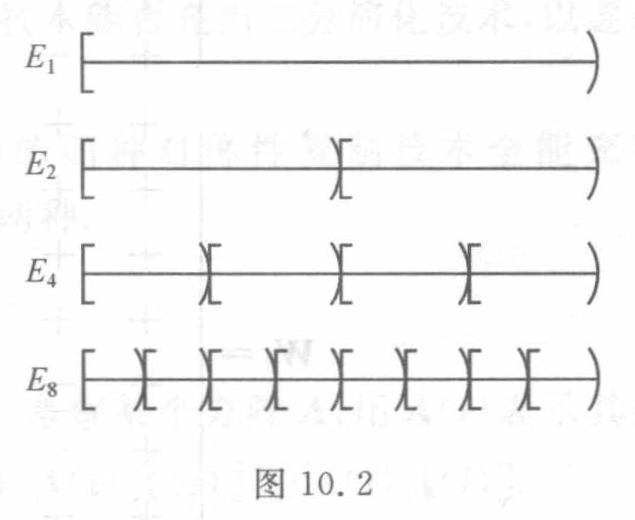
\includegraphics[width=0.85\linewidth,height=\textheight,keepaspectratio,alt={图 10.2（原图裁切）：时基上的二分集}]{../assets/ch10/fig-10-2.png}

图 10.2

\begin{quote}
图中文字与图意（转录）：四行标号为 \(E_1\)、\(E_2\)、\(E_4\)、\(E_8\)，每行表示左闭右开的子段，按行依次二分。
\end{quote}

现在的问题是，如何在二分集的各个子段上布值 \(+1\) 与 \(-1\) 以设计出一个完备的正交函数系？实际上，这种函数系就是 Walsh 函数系。

为规范起见，约定 Walsh 函数第一个阶跃值（即最左侧的子段上的函数值）为 \(+1\)，如图 10.1 所示。

在形形色色的 Walsh 函数中，最简单的自然是\textbf{方波}

\[
R(x)=1,\quad0\leqslant x<1.
\]

然而这个函数过于平凡而显得``空虚''，其中似乎不含任何信息。``波''的含义是波动、起伏。按这种理解，时基上的方波似乎不能算作真正的``波''。具有波动性的最简单的

\href{../../source-images/pdf-265.jpeg}{原页}

波形是下列 \textbf{Haar 波}：

\[
H(x)=\begin{cases}
+1,&0\leqslant x<\dfrac12,\\[4pt]
-1,&\dfrac12\leqslant x<1.
\end{cases}
\]

由图 10.1 知，方波与 Haar 波是 Walsh 函数系的源头。

\subsubsection{10.2.2　Walsh 函数的矩阵表示}\label{walsh-ux51fdux6570ux7684ux77e9ux9635ux8868ux793a}

Walsh 函数仅取 \(+1\) 与 \(-1\) 两个值。为简约起见，后文常将 \(+1\) 与 \(-1\) 简记为``\(+\)''与``\(-\)''。

由于 Walsh 函数在二分集的每个子段上取值 \(+\) 或 \(-\)，因而它们可表示为某个向量，而第 \(n\) 族 Walsh 函数的全体则可表达为一个 \(N=2^n\) 阶方阵，称作 \textbf{Walsh 方阵}。

据图 10.1 容易看出，前面几个 Walsh 方阵分别是

\[
W_1=[\,+\,],
\]

\[
W_2=\begin{pmatrix}+&+\\+&-\end{pmatrix},
\]

\[
W_4=\begin{pmatrix}
+&+&+&+\\
+&+&-&-\\
+&-&-&+\\
+&-&+&-
\end{pmatrix},
\]

\[
W_8=\begin{pmatrix}
+&+&+&+&+&+&+&+\\
+&+&+&+&-&-&-&-\\
+&+&-&-&-&-&+&+\\
+&+&-&-&+&+&-&-\\
+&-&-&+&+&-&-&+\\
+&-&-&+&-&+&+&-\\
+&-&+&-&-&+&-&+\\
+&-&+&-&+&-&+&-
\end{pmatrix}.
\]

请读者据图 10.1 列出 Walsh 方阵 \(W_{16}\)。

Walsh 方阵看上去是个复杂系统，这个复杂系统中究竟潜藏着怎样的规律性呢？

\end{document}
